\chapter{三角函数的性质与图象}

在展开本章具体内容之前,首先应明确两点:(1)研究函数性质的依据是函数的定义。对于三角函数来讲,它的每种函数的定义与其相应的三角函数线的定义是彼此等价的(一种是代数形式,一种是几何形式、代数形式便于计算,几何形式形象直观). 因此,研究中根据需要我们可以灵活地选用任何一种形式;(2)在中学阶段,研究\textbf{函数的初等性质}主要限于以下五个方面:
\begin{enumerate}
    \item 定义域(我们用$D$表示它);
    \item 值域(对$D$而言,是整体性质);
    \item 增减性(对$D$的某个子区间而言,是局部性质),
    \item 奇偶性(对$D$而言,是整体性质);
    \item 周期性(对$D$而言,是整体性质)。
\end{enumerate}

在1.4节,我们曾经利用单位圆,对三角函数的某些性质(定义域、值域、五组诱导公式)做过初步的探究。本章将在此基础上完成对三角函数初等性质的全面研究,并画出各种三角函数的图象。

\section{关于三角函数定义域与值域的补充}

{练习}:
 根据三角函数(或三角函数线)的定义填表:
\begin{center}
\begin{tabular}{c|c|c|c|c|c|c}
\hline
函数 & $\sin\alpha=y$&$\cos\alpha=x$& $\tan\alpha=\frac{y}{x}$&$\cot\alpha=\frac{x}{y}$&$\sec\alpha=\frac{1}{x}$&$\csc\alpha=\frac{1}{y}$\\
\hline
定义域&&&&&\\
\hline
值域&&&&&\\
\hline
\end{tabular}
\end{center}    

\begin{example}
    求下列函数的定义域。
\begin{multicols}{2}
\begin{enumerate}[(1)]
    \item $f(\alpha)=\sqrt{\cot\alpha\cdot\csc\alpha}$
    \item $f( \beta ) = \sqrt {\sin \beta }+\lg(2\cos\beta+1)$
    \item $f( x) = \frac {\sin x\cdot \tan \left ( x- \frac \pi 4\right ) }{2\cos x- 1}$
\end{enumerate}    
\end{multicols}

\end{example}

\begin{solution}
\begin{enumerate}[(1)]
    \item 要 使 $f( \alpha )$ 有意义,须$\cot \alpha\cdot\csc\alpha\ge 0$, 即$\cot\alpha$与$\csc\alpha$同号或积为零。在图 3.1 中我们分别标出这两个函数值的符号。“可见动点应落在实线画出的弧上(注意:点$B$、$C$在
内,点$A$除外),

$\therefore\quad \alpha\in\left(0+2k\pi,\; \frac{\pi}{2}+2k\pi\right]\cup\left[\frac{3\pi}{2}+2k\pi,\; 2\pi+2k\pi\right),\quad k\in\Z$

\noindent
\begin{minipage}{.45\textwidth}
\centering
\begin{tikzpicture}[>=stealth]
\draw[->](-2.5,0)--(2.5,0)node[below]{$x$};
\draw[->](0,-2.5)--(0,2.5)node[left]{$y$};
\draw(0,-1.5) arc (-90:90:1.5);
\draw[dashed](0,1.5) arc (90:270:1.5);
\foreach \x in {1.5, -1.5}
{
    \draw[fill=white] (\x,0)circle(1.5pt);
    \draw[fill] (0,\x)circle(1.5pt);
}
\node at (1.5,0)[above right]{$A$};
\node at (0,1.5)[above right]{$C$};
\node at (0,-1.5)[below right]{$B$};
\node [below left]{$O$};
\node at (.5,.75)[text width=1cm, align=center]{$+$\\$+$};
\node at (-.5,.75)[text width=1cm, align=center]{$-$\\$+$};
\node at (.5,-.75)[text width=1cm, align=center]{$-$\\$-$};
\node at (-.5,-.75)[text width=1cm, align=center]{$+$\\$-$};

\end{tikzpicture}   
\captionof{figure}{} 
\end{minipage}\hfill
\begin{minipage}{.45\textwidth}
\centering
\begin{tikzpicture}[>=stealth]
\draw[->](-2.5,0)--(2.5,0)node[below]{$x$};
\draw[->](0,-2.5)--(0,2.5)node[left]{$y$};
\draw(0,0)node[below right]{$O$}circle (1.5);
\draw[dashed](-0.75,-2.5)--(-0.75,2.5);
\draw[thick](120:1.5)--(0,0)--(-120:1.5);
\draw[fill=white] (120:1.5)node[above left]{$P$}  circle(1.5pt);
\draw[fill=white] (-120:1.5)node[below left]{$Q$}  circle(1.5pt);
\draw[->, thick](0,0)--(-.75,0)node[below left]{$N$};
\node at (1.5,0)[below right]{$A$};
\draw[->](.35,0) arc (0:120:.35);
\node at (60:.6){$\tfrac{2\pi}{3}$};

\end{tikzpicture}    
\captionof{figure}{} 

\end{minipage}


\item 要使$f(\beta)$有意义,须
\begin{align}
    \sin\beta\ge 0 \tag{1}\\
    2\cos\beta +1>0\Longleftrightarrow \cos\beta>-\frac{1}{2}\tag{2}
\end{align}
在单位圆上(图3.2)画出余弦线$\VEC{ON}=-\frac{1}{2}$,过$N$作$PQ\parallel y$轴,则满足(2)的动点应落在$\widearc{QAP}$上,满足(1)的动点应落在$x$轴(含$x$轴)上方的弧上. 从而,满足 不等式(1)(2)的动点应落在$\widearc{AP}$上.

$\therefore\quad \beta\in \left[0+2k\pi,\; \frac{2\pi}{3}+2k\pi\right),\quad k\in\Z$

\item 要使$f(x)$有意义,须
\[\begin{cases}
    x-\frac{\pi}{4}\ne\frac{\pi}{2}+k\pi\Longleftrightarrow x\ne \frac{3\pi}{4}+k\pi\quad (k\in\Z)\\
    \cos x\ne \frac{1}{2}
\end{cases}\]
在单位圆上,满足不等式组的$x$的对应点应落在图3.3中实线画出的弧上,即$x\in\R$,且$x\ne \frac{3\pi}{4}+k\pi$,$x\ne \frac{\pi}{3}+2k\pi$,$x\ne \frac{5\pi}{3}+2k\pi\; (k\in\Z)$,或者表示成
\[\begin{split}
x\in &\left(\frac{\pi}{3}+2k\pi,\; \frac{3\pi}{4}+2k\pi\right)\cup \left(\frac{3\pi}{4}+2k\pi,\; \frac{5\pi}{3}+2k\pi\right)\\
&\cup \left(\frac{5\pi}{3}+2k\pi,\; \frac{7\pi}{4}+2k\pi\right)\cup \left(-\frac{\pi}{4}+2k\pi,\; \frac{\pi}{3}+2k\pi\right),\quad k\in\Z
\end{split}\]

\noindent
\begin{minipage}{.45\textwidth}
    \centering
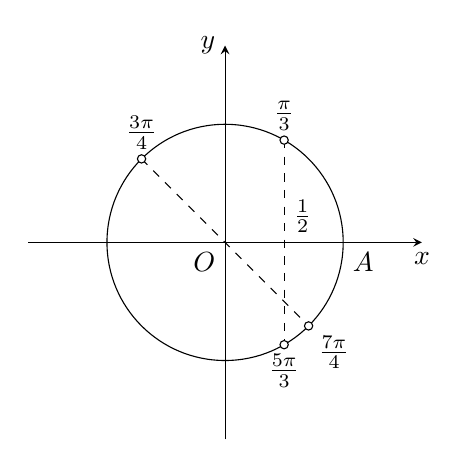
\begin{tikzpicture}[>=stealth]
    \draw[->](-2.5,0)--(2.5,0)node[below]{$x$};
    \draw[->](0,-2.5)--(0,2.5)node[left]{$y$};
    \draw(0,0)node[below left]{$O$}circle (1.5);
    \draw[dashed] (60:1.5)node[above]{$\frac{\pi}{3}$}--(-60:1.5)node[below]{$\frac{5\pi}{3}$};
    \draw[dashed] (135:1.5)node[above]{$\frac{3\pi}{4}$}--(-45:1.5)node[below right]{$\frac{7\pi}{4}$};
\foreach \x in {60,-60,135,-45}
{
    \draw[fill=white](\x:1.5) circle(1.5pt);
}
\node at (.75,0)[above right]{$\frac{1}{2}$};
\node at (1.5,0)[below right]{$A$};
\end{tikzpicture}
    \captionof{figure}{}
\end{minipage}
\hfill
\begin{minipage}{.45\textwidth}
    \centering
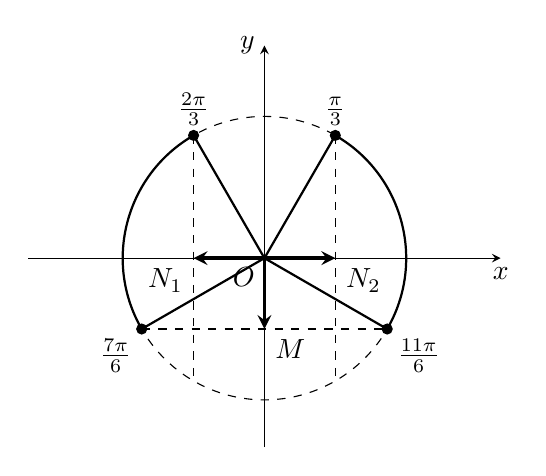
\begin{tikzpicture}[>=stealth, scale=1.2]
    \draw[->](-2.5,0)--(2.5,0)node[below]{$x$};
    \draw[->](0,-2)--(0,2.25)node[left]{$y$};
    \draw[dashed](0,0)node[below left]{$O$}circle (1.5);
    \draw[dashed] (60:1.5)node[above]{$\frac{\pi}{3}$}--(-60:1.5);
    \draw[dashed] (120:1.5)node[above]{$\frac{2\pi}{3}$}--(-120:1.5);
\foreach \x in {60,-30,120,-150}
{
    \draw[fill](\x:1.5) circle(1.5pt);
    \draw[thick](\x:1.5)--(0,0);
}
\draw[thick](-30:1.5)node[below right]{$\frac{11\pi}{6}$} arc (-30:60:1.5);
\draw[thick](210:1.5)node[below left]{$\frac{7\pi}{6}$} arc (210:120:1.5);
\draw[dashed](210:1.5)--(-30:1.5);
\draw[very thick,->](0,0)--(0,-.75)node[below right]{$M$};
\draw[very thick,->](0,0)--(-.75,0)node[below left]{$N_1$};
\draw[very thick,->](0,0)--(.75,0)node[below right]{$N_2$};
\end{tikzpicture}
\captionof{figure}{}
\end{minipage}


\end{enumerate}
\end{solution}

\begin{example}
    解不等式组:
\begin{align}
    \sin x>-\frac{1}{2} \tag{1}\\
    |\cos x|\ge \frac{1}{2}\tag{2}
\end{align}
\end{example}

\begin{solution}
在单位圆上分别作出正弦线$\VEC{OM}=-\frac{1}{2}$,余弦线$\VEC{ON_1}=-\frac{1}{2}$,$\VEC{ON_2}=\frac{1}{2}$,过点$M$、$N_1$、$N_2$分别作$x$轴和$y$轴的平行线(图3.4)。可知满足不等式组的动点应落在实线画出的弧上,从而有
\[x\in\left[\frac{2\pi}{3}+2k\pi,\; \frac{7\pi}{6}+2k\pi\right)\cup \left(-\frac{\pi}{6}+2k\pi,\; \frac{\pi}{3}+2k\pi\right],\quad k\in\Z\]

\end{solution}

\begin{thm}{思考题}
    上式中后一个区间写成下面的形式,错在哪里?
\[\left(\frac{11\pi}{6}+2k\pi,\; \frac{\pi}{3}+2k\pi\right),\quad k\in\Z\]
\end{thm}

\begin{example}
   写出使下列不等式成立的$x$的集合: 
\begin{multicols}{2}
\begin{enumerate}[(1)]
    \item  $\sqrt{3}+\tan x\leq 0$
    \item $\cot x-2\geqslant 0$ 
\end{enumerate}
\end{multicols}
\end{example}

\begin{solution}
\begin{enumerate}[(1)]
    \item 由原式,得$\tan x\leqslant-\sqrt{3}$,

$\therefore\quad x\in \left ( \frac \pi 2+ k\pi , \frac {2\pi }3+ k\pi \right ],\; k\in \Z$(图3.5).

\noindent
\begin{minipage}{.45\textwidth}
\begin{tikzpicture}[>=stealth]
\draw[->](-2.5,0)--(2.5,0)node[below]{$x$};
\draw[->](0,-2.5)--(0,2.5)node[left]{$y$};
\node [below left]{$O$};
\node at (1.5,0)[below right]{$A$};
\draw[dashed](0,0) circle(1.5);
\draw(1.5,0)--(1.5,-1.5*1.732)node[below]{$\sqrt{3}$};
\draw[dashed](120:1.5)node[above left]{$\frac{2\pi}{3}$}--(1.5,-1.5*1.732);
\draw[very thick](0,1.5) arc (90:120:1.5);
\draw[very thick](0,-1.5) arc (-90:-60:1.5)node[below]{$\frac{5\pi}{3}$};
\draw[fill=white](0,-1.5)circle(1.5pt);
\draw[fill=white](0,1.5)circle(1.5pt);
\draw[fill](120:1.5)circle(1.5pt);
\draw[fill](-60:1.5)circle(1.5pt);
\end{tikzpicture}    
\captionof{figure}{}
\end{minipage}\hfill
\begin{minipage}{.45\textwidth}
\begin{tikzpicture}[>=stealth]
\draw[->](-2.5,0)--(2.5,0)node[below]{$x$};
\draw[->](0,-2.5)--(0,2.5)node[left]{$y$};
\node [below right]{$O$};
\node at (1.5,0)[below right]{$A$};
\draw[dashed](0,0) circle(1.5);
\draw(0,1.5)--(3,1.5)node[right]{2};
\draw[dashed](-180+26.56:1.5)node[below left]{$\pi+x'$}--(3,1.5);
\draw[very thick](1.5,0) arc (0:26.56:1.5)node[right]{$x'$};
\draw[very thick](-1.5,0) arc (180:206.56:1.5);
\draw[fill=white](-1.5,0)circle(1.5pt);
\draw[fill=white](1.5,0)circle(1.5pt);
\draw[fill](26.56:1.5)circle(1.5pt);
\draw[fill](-180+26.56:1.5)circle(1.5pt);

\end{tikzpicture}    
\captionof{figure}{}
\end{minipage}

\item 由原式,得
$\cot x\ge 2$,对于$x$的边界值$x'$来说,$\cot x'=2$不是特殊角,我们可以用量角器量出$x'$的值(在精度要求不高的情况下,这样做是可行的),从而
$x\in (0+k\pi,\; x'+k\pi],\quad k\in\Z$(图3.6)。
\end{enumerate}
\end{solution}

\begin{remark}
求三角函数式的定义域,归结为解三角不等式(或不等式组)。可以先在周内角范围内运用三角函数线进行研究,然后再考虑一般情况。
\end{remark}

\begin{thm}
    {思考题} 你能说出下列三角函数的值域吗?
\begin{multicols}{3}
\begin{enumerate}[(1)]
    \item $y=\sin x+3$
    \item $y=2\cos x$
    \item $y=-3\sin x+1$
\end{enumerate}    
\end{multicols}
\end{thm}

\begin{example}
试求函数$f(x)=\sin x+\cos x$的值域。
\end{example}

\begin{thm}
  {问1}由$-1\le \sin x\le 1$, $-1\le \cos x\le 1$, $f(x)$的值域是否为$[-2,2]$呢?
\end{thm}

\begin{analyze}
$f(x)$的值域不是$[-2,2]$。这是因为当$\sin x$取得最小值$-1$时,$x=-\frac{\pi}{2}+2k\pi,\; (k\in\Z)$,此时$\cos x$并不能取得最小值$-1$.对于$\sin x$取最大值的情况也是类似的。因此,欲求$f(x)$的值域,应先化简$f(x)$.
\end{analyze}

\begin{solution}
    根据$a\sin x +b\cos x$的化积公式,有
\[f(x)=\sin x+\cos x=\sqrt{2} \sin\left(x+\frac{\pi}{4}\right)\]

$\because\quad -1\le \sin\left(x+\frac{\pi}{4}\right)\le 1$

$\therefore\quad -\sqrt{2}\le \sqrt{2}\sin\left(x+\frac{\pi}{4}\right)\le \sqrt{2}$

即,$f(x)$的值域为$\left[-\sqrt{2},\; \sqrt{2}\right]$.
\end{solution}

\section*{习题一}
\begin{center}
    \bfseries A
\end{center}

\begin{enumerate}
    \item (口答)求下列 函数 的定义域:
\begin{multicols}{2}
\begin{enumerate}[(1)]
    \item $f(x)=\frac{1}{1+\sin x}$
    \item $f(x)=\frac{1}{1-\cos x}$
    \item $f(x)=\sqrt{\cos x}$
    \item $f(x)=\sqrt{-2\sin x}$
\end{enumerate}
\end{multicols}
\item 求下列 函数 的定义域:
\begin{multicols}{2}
\begin{enumerate}[(1)]
    \item $y=-\tan\left(x+\frac{\pi}{6}\right)+2$
    \item $y=\cot\left(x+\frac{\pi}{3}\right)$
    \item $y=\tan\frac{x}{2}$
    \item $y=2\cot\left(2x-\frac{\pi}{3}\right)$
    \item $y=\frac{1}{1-\tan x}$
    \item $y=\frac{\cot x}{\cos x -\frac{1}{2}}$
\end{enumerate}
\end{multicols}
\item 求下列 函数 的定义域:
\begin{multicols}{2}
\begin{enumerate}[(1)]
\item $f(t)=\tan t\cdot \cot t$
\item $f(t)=\cos t\cdot \sec t$
\item $f(t)=\sqrt{-\cos t}-\lg\sin t$
\end{enumerate}
\end{multicols}

\item 解不等式:
\begin{multicols}{2}
\begin{enumerate}[(1)]
    \item $\sin x\ge \frac{\sqrt{3}}{2}$
    \item $\sqrt{2}+2\cos x\ge 0$
    \item $1+\tan x\ge 0$
    \item $\cot x-\sqrt{3}\ge 0$
    \item $\tan x-3\le 0$
    \item $2\cot x+3\ge 0$
\end{enumerate}
\end{multicols}

\item 下列各式能不能成立?为什么?
\begin{multicols}{2}
\begin{enumerate}[(1)]
    \item $\cos^2 x=\frac{3}{2}$
    \item $\sin^3 x=-\frac{\pi}{4}$
    \item $\sin x+\cos x=2$
    \item $\tan x+\cot x=2$
\end{enumerate}
\end{multicols}

\item 试求下列函数的值域:
\begin{multicols}{2}
\begin{enumerate}[(1)]
    \item $y=5\sin x$
    \item $y=\cos x -4$
    \item $y=-2\sin x+6$
    \item $y=\cos\left(3x+\frac{\pi}{4}\right)$
    \item $y=\sin x-\cos x$
    \item $y=a\sin x+b\cos x$
    \item $y=\sin^2x-\sin x+\frac{\pi}{4}$
    \item $y=\cos^2 x+6\cos x+10$
\end{enumerate}
\end{multicols}
\end{enumerate}

\begin{center}
    \bfseries B
\end{center}
\begin{enumerate}\setcounter{enumi}{6}
    \item 求函数$f(t)$的定义域:
\[f(t)=\sqrt{-4\sin^2 t+2(1+\sqrt{3})\sin t-\sqrt{3}}\]
\end{enumerate}

\begin{center}
    \bfseries C
\end{center}
\begin{enumerate}\setcounter{enumi}{7}
    \item 当$a$为何实数值 时,下列 函数的定义 域是$\R$?
\[f(x)=\sqrt{\sin^6 x+\cos^6 x+a\sin x\cos x}\]
\end{enumerate}

\section{三角函数的增减性}
利用三角函数线,研究三角函数值的增、减变化的规律是形象、简捷的。

\subsection{$f(\alpha)=\sin\alpha,\; \alpha\in\R$}
从图3.7可见,当动点$P$从点$B_1$逆时针转动到点$B$时,正弦值从$-1$逐渐增加到$+1$; 当动点$P$从$B$逆时针转动到$B_1$时,正弦值又从$+1$逐渐减少到$-1$。由此,正弦函数的
\begin{itemize}
    \item 增区间为$\left[-\frac{\pi}{2}+2k\pi,\; \frac{\pi}{2}+2k\pi\right],\quad k\in\Z$;
    \item 减区间为$\left[\frac{\pi}{2}+2k\pi,\; \frac{3\pi}{2}+2k\pi\right],\quad k\in\Z$.
\end{itemize}

\subsection{$f(\alpha)=\cos\alpha,\; \alpha\in\R$}

从图3.8可见,当动点$P$从$A_1$逆时针转动到点$A$时,余弦值从$-1$逐渐增加到$+1$,当动点$P$从$A$逆时针转动到$A_1$点时,余弦值又从$+1$逐渐减少到$-1$.由此,余弦函数的
\begin{itemize}
    \item 增区间为$\left[\pi+2k\pi,\; 2\pi+2k\pi\right],\quad k\in\Z$;
    \item 减区间为$\left[0+2k\pi,\; \pi+2k\pi\right],\quad k\in\Z$.
\end{itemize}


\begin{example}
    
\end{example}

\begin{analyze}
    
\end{analyze}

\begin{solution}
    
\end{solution}



\begin{example}
    
\end{example}

\begin{analyze}
    
\end{analyze}

\begin{solution}
    
\end{solution}



\begin{example}
    
\end{example}

\begin{analyze}
    
\end{analyze}

\begin{solution}
    
\end{solution}



\begin{example}
    
\end{example}

\begin{analyze}
    
\end{analyze}

\begin{solution}
    
\end{solution}



\begin{example}
    
\end{example}

\begin{analyze}
    
\end{analyze}

\begin{solution}
    
\end{solution}



\begin{example}
    
\end{example}

\begin{analyze}
    
\end{analyze}

\begin{solution}
    
\end{solution}



\begin{example}
    
\end{example}

\begin{analyze}
    
\end{analyze}

\begin{solution}
    
\end{solution}



\begin{example}
    
\end{example}

\begin{analyze}
    
\end{analyze}

\begin{solution}
    
\end{solution}



\begin{example}
    
\end{example}

\begin{analyze}
    
\end{analyze}

\begin{solution}
    
\end{solution}



\begin{example}
    
\end{example}

\begin{analyze}
    
\end{analyze}

\begin{solution}
    
\end{solution}



\begin{example}
    
\end{example}

\begin{analyze}
    
\end{analyze}

\begin{solution}
    
\end{solution}



\begin{example}
    
\end{example}

\begin{analyze}
    
\end{analyze}

\begin{solution}
    
\end{solution}



\begin{example}
    
\end{example}

\begin{analyze}
    
\end{analyze}

\begin{solution}
    
\end{solution}



\begin{example}
    
\end{example}

\begin{analyze}
    
\end{analyze}

\begin{solution}
    
\end{solution}



\begin{example}
    
\end{example}

\begin{analyze}
    
\end{analyze}

\begin{solution}
    
\end{solution}



\begin{example}
    
\end{example}

\begin{analyze}
    
\end{analyze}

\begin{solution}
    
\end{solution}



\begin{example}
    
\end{example}

\begin{analyze}
    
\end{analyze}

\begin{solution}
    
\end{solution}



\begin{example}
    
\end{example}

\begin{analyze}
    
\end{analyze}

\begin{solution}
    
\end{solution}



\begin{example}
    
\end{example}

\begin{analyze}
    
\end{analyze}

\begin{solution}
    
\end{solution}



\begin{example}
    
\end{example}

\begin{analyze}
    
\end{analyze}

\begin{solution}
    
\end{solution}



\begin{example}
    
\end{example}

\begin{analyze}
    
\end{analyze}

\begin{solution}
    
\end{solution}



\begin{example}
    
\end{example}

\begin{analyze}
    
\end{analyze}

\begin{solution}
    
\end{solution}



\begin{example}
    
\end{example}

\begin{analyze}
    
\end{analyze}

\begin{solution}
    
\end{solution}



\begin{example}
    
\end{example}

\begin{analyze}
    
\end{analyze}

\begin{solution}
    
\end{solution}


























